\documentclass[border=14pt]{standalone}
\usepackage[T1]{fontenc}
\usepackage[scaled]{helvet}
\renewcommand\familydefault\sfdefault
\usepackage{tikz}
\usetikzlibrary{arrows.meta,calc,positioning}
\definecolor{personF}{HTML}{F8E0A8}\definecolor{personD}{HTML}{B8860B}
\definecolor{slackF}{HTML}{DCE8F6}\definecolor{slackD}{HTML}{5B7FA8}
\definecolor{sessF}{HTML}{CDE8E1}\definecolor{sessD}{HTML}{2E8B74}
\definecolor{subF}{HTML}{E6DDF3}\definecolor{subD}{HTML}{7E5DB8}
\definecolor{workF}{HTML}{E1EECD}\definecolor{workD}{HTML}{6A9A3A}
\definecolor{servF}{HTML}{E6E8EB}\definecolor{servD}{HTML}{8A9099}
\definecolor{codeF}{HTML}{F6DAD6}\definecolor{codeD}{HTML}{C0605A}
\definecolor{arrC}{HTML}{6B7280}\definecolor{labC}{HTML}{555B66}
\tikzset{
  box/.style={rounded corners=3pt, draw, line width=0.8pt, align=center, text width=3.4cm,
              inner sep=5pt, minimum height=1.2cm, font=\normalsize},
  person/.style={box, fill=personF, draw=personD},
  slack/.style={box, fill=slackF, draw=slackD},
  sess/.style={box, fill=sessF, draw=sessD},
  sub/.style={box, fill=subF, draw=subD},
  work/.style={box, fill=workF, draw=workD},
  serv/.style={box, fill=servF, draw=servD},
  code/.style={box, fill=codeF, draw=codeD},
  arr/.style={-{Stealth[length=2.4mm,width=1.8mm]}, draw=arrC, line width=0.8pt},
  lab/.style={font=\small\itshape, text=labC, fill=white, inner sep=1.5pt},
}
\hyphenpenalty=10000 \exhyphenpenalty=10000
\newcommand\nd[2]{\textbf{#1}\\[1pt]{\small #2}}
\newcommand\titled[2]{\node[anchor=south west, inner sep=0pt] at ($(current bounding box.north west)+(0cm,0.45cm)$)
  {{\bfseries\LARGE #1}\hspace{1.2em}{\color{labC}\large #2}};}
\begin{document}
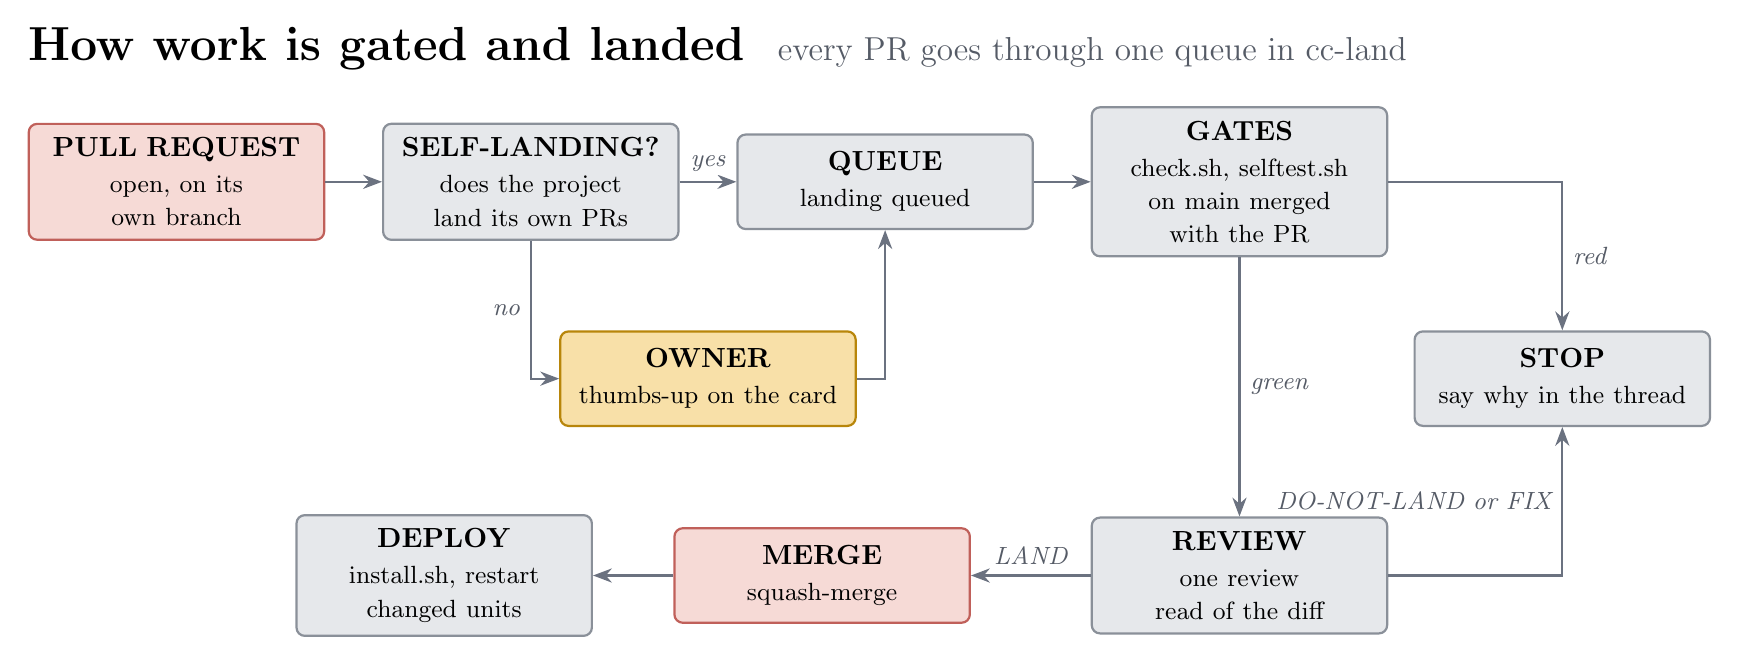
\begin{tikzpicture}
\node[code] (pr) at (0,0) {\nd{PULL REQUEST}{open, on its own branch}};
\node[serv] (q) at (4.5,0) {\nd{SELF-LANDING?}{does the project land its own PRs}};
\node[serv] (queue) at (9,0) {\nd{QUEUE}{landing queued}};
\node[serv] (gates) at (13.5,0) {\nd{GATES}{check.sh, selftest.sh on main merged with the PR}};
\node[person] (up) at (6.75,-2.5) {\nd{OWNER}{thumbs-up on the card}};
\node[serv] (stop) at (17.6,-2.5) {\nd{STOP}{say why in the thread}};
\node[serv] (rev) at (13.5,-5) {\nd{REVIEW}{one review read of the diff}};
\node[code] (merge) at (8.2,-5) {\nd{MERGE}{squash-merge}};
\node[serv] (dep) at (3.4,-5) {\nd{DEPLOY}{install.sh, restart changed units}};
\draw[arr] (pr) -- (q);
\draw[arr] (q) -- node[lab, above=2pt] {yes} (queue);
\draw[arr] (q.south) |- node[lab, pos=0.25, left=2pt] {no} (up.west);
\draw[arr] (up.east) -| (queue.south);
\draw[arr] (queue) -- (gates);
\draw[arr] (gates.east) -| node[lab, pos=0.75, right=2pt] {red} (stop.north);
\draw[arr] (gates) -- node[lab, right=2pt] {green} (rev);
\draw[arr] (rev.east) -| node[lab, pos=0.75, left=2pt] {DO-NOT-LAND or FIX} (stop.south);
\draw[arr] (rev) -- node[lab, above=2pt] {LAND} (merge);
\draw[arr] (merge) -- (dep);
\titled{How work is gated and landed}{every PR goes through one queue in cc-land}
\end{tikzpicture}
\end{document}
